\documentclass{article}

% author: Filipe Funenga

\usepackage{amsmath}
\usepackage{amsfonts}
\usepackage{amsthm}
\newtheorem{problem}{Problem}
\newtheorem{lemma}{Lemma}
\usepackage{eurosym}
\usepackage{fullpage}
\usepackage{hyperref}
\usepackage{graphicx}
%\usepackage[pagewise]{lineno}
%\linenumbers

\begin{document}
\title{Introduction to the Betting Exchange}
\author{Filipe Funenga\\
\texttt{filipe.funenga@ist.utl.pt}\\
Lisbon,Portugal}
\date{September 18, 2012}
\maketitle
\begin{center} {\small \bf Keywords:} betting exchange, betfair,
                                        trading, back, lay \end{center}
\begin{abstract}
A basic introduction is made to trading in a betting exchange. 
Beyond analysing the central system of equations for trading in its 
matrix form, an equation is provided aiming at a dynamic 
configuration of the proportion between returns. Also, various 
approaches are presented, denoting the possibility for a trader to 
manage the profits based on his expectation of the event.
\end{abstract}
\tableofcontents
\section{Betting Exchange}
An online betting exchange is a web service where users can, among 
other things, trade contracts with each other about the outcome of 
future random events. The pay-off of these contracts can either be 
some fixed amount of money or nothing at all. The main innovation of 
this system, compared to traditional bookmakers, lies in providing a 
method to set fixed odds against an outcome | known as \emph{laying} 
| and invite other users to bet in favour of the outcome | know as 
\emph{backing}. This type of freedom had previously been reserved 
only to bookmakers.

The betting exchange concept, envisioned and created by 
Betfair\textsuperscript{\textregistered} in 2000, has revolutionized 
sports and race wagering, attracting the attention of sports bodies, 
major competitors and governments, who seem uncertain about how to 
deal with this revolutionary transaction system, as well as 
customers globally, who are attracted by the far superior value 
proposition offered. \cite{DaviesPittShapiroWatson2005} Smaller 
companies exist but Betfair\textsuperscript{\textregistered} is 
considered to have a virtual monopoly.

In facilitating betting as a neutral intermediary the company 
responsible for maintaining the exchange generates revenue by taking 
a commission from the winner of the contract. This means that the 
company is only interested in maximizing the amount of money 
transacted between users and that it has no vested interest in the 
outcome of the events. The commission charged is calculated as a 
percentage of net winnings for each customer on each event, or 
market. The final value that the customer will get can be calculated 
with the \emph{house function}, $H$, which is formulated in the 
following manner:

\begin{equation}
\label{eq:commision}
    H(x) = \left\{
    \begin{array}{l l}
        x              & \quad \text{if x $\leq$ 0}\\
        x \times (1-h) & \quad \text{if x $>$ 0}\\
    \end{array} \right.
\end{equation}
where $h$ is the house percentage (normally $0.05$).

The neutral position makes customers, whose betting activities have 
traditionally been "restricted" by bookmakers (normally successful 
users that won too much money), able to place bets only limited by 
market liquidity. \cite{laffey2005}

\section{Decimal Odds and Probabilities}
\label{sec:decimalOddsAndProbabilities}
Traditional odds in favour of an event, $O_{t}$, is the ratio of the 
probability that an event will happen to the probability that it 
will not happen. For example, the traditional odds that a randomly 
chosen day of the week is a Sunday are one to six, which is written 
$1/6$ or 1:6. 

Decimal Odds, $O_{d}$, are simpler to use than traditional ones and 
are the most common form of odds quoted in countries outside the UK. 
Unlike the traditional interpretation, the customer stake is 
included as part of his total return, $O_{t}=O_{d}+1$, relating more 
closely to the concept of probability. In the previous example, each 
day of the week has decimal odds of 7.0.

The implied probability of an outcome described by decimal odds, 
equals 1 divided by its odds:

\[
\text{Probability}=\frac{1}{O_{d}}=\frac{1}{O_{t}-1}
\]
which concludes that everyday there is a $\frac{1}{7} = 14.3\%$ 
chance of being Sunday.

This means that when a customer makes a bet, he is actually making a 
financial commitment about his expectations on the outcome of an 
event through the implied probability of the bet. As we will see in 
appendix \ref{apdx:expectedvariance}, the expected value of bets 
depend on a relation between the real probability of the event and 
the implicit probability of the bet.

\section{Betting Terminology}
Various terms are nowadays well established to characterize the way 
betting exchange's customers build their sets of bets.

First of all, clear distinctions arise related to the number of 
betted events. If the set only backs and/or lays one event, than it 
is said that the costumer is \emph{Hedging}. On the contrary, if 
more than one event is betted upon, than its called \emph{Dutching}.

A particular case of \emph{Hedging} is when the costumer only closes 
one bet. This sort of action is known as \emph{Speculating} since 
the costumer's (colloquially called a \emph{punter}) transactions 
are based on hints. For instance, a \emph{punter} will easily close 
a back bet on a single event of a soccer game and wait until the end 
to see the outcome.

\emph{Dutching} also has a special case called \emph{Surebeting}. 
This happens when the events betted upon are collectively exhaustive 
(all the possible events).

\begin{center}
    \begin{tabular}{ | c | c |}
        \hline
        Number o Betted Events & Terminology \\ \hline\hline
        Single & \emph{Hedging} of \emph{Speculating}\\ \hline
        Multiple & \emph{Dutching} or \emph{Surebeting}\\
        \hline
    \end{tabular}
\end{center}

The closing of bets can be further distinguished based on its 
timing, denoting two well known fashions: \emph{Arbitrage} and
\emph{Trading}.

In economics and finance, \emph{Arbitrage} is the practice of taking 
advantage of a price difference between two or more markets: 
striking a combination of matching deals that capitalize upon the 
imbalance, the profit being the difference between the market prices.

In the betting exchange context, it is possible to became an 
\emph{Arbitrageur} when the implied probabilities (see 
\ref{sec:decimalOddsAndProbabilities}) of all possible events sum up to 
more than one. For instance, in a soccer match the odds available 
for backing $\{\text{Home},\text{Visitor},\text{Draw}\}$ are $O_{i} 
= \{1.3, 4.3, 2.3\}$, respectively. This results in a total 
$\sum_{i} \frac{1}{O_{i}} = 1.44$ probability which now allows to 
take profit with a \emph{Surebet}. \emph{Arbitrageurs} are 
traditionally known to perform \emph{surebets} on multiple 
bookmakers. The same situation can be performed, although highly 
unlikely, with hedging. 

A \emph{Trader}, someone who performs \emph{Trading}, takes an extra 
risk and closes his bets at different stages when the implied 
probabilities offered by the market turn out to be more favourable.

\begin{center}
    \begin{tabular}{ | c | c |}
        \hline
        Generation of Imbalance & Terminology \\ \hline\hline
        Immediate & \emph{Trading}\\ \hline
        Gradual & \emph{Arbitrage}\\
        \hline
    \end{tabular}
\end{center}

\section{The Back-Lay Pair}
The profit/loss of back and lay bets can be represented as random 
variables established by a stake and an implied probability in the 
following manner:

\[
\begin{array}{r c l}
    Back( p_{B}, s_{B} ) & = & \left\{
    \begin{array}{l l}
        s_{B} \times \frac{1-p_{B}}{p_{B}} & \quad
                                           \text{if the event occurs}\\
        s_{B} \times (-1)                  & \quad
                                                 \text{if it doesn't}\\
    \end{array} \right. \\
    
    Lay( p_{L}, s_{L} ) & = & \left\{
    \begin{array}{l l}
        s_{L} \times \frac{p_{L}-1}{p_{L}} & \quad
                                           \text{if the event occurs}\\
        s_{L}                              & \quad
                                                 \text{if it doesn't}\\
    \end{array} \right.
\end{array}
\]
where $p_{B}$ and $p_{L}$ are the implied probabilities of the bet, 
$s_{B}$ and $s_{L}$ the stakes. The expected value and variance of 
each variable are calculated in \ref{apdx:expectedvariance}.

Nowadays, in order to understand if it is possible to make profit 
with this pair of bets, the most common metric used is the 
\emph{greenbook} which is defined has the situation of having 
positive profits in all markets (regardless to the distribution). 
Although this is an acceptable way of evaluating the established 
situation, a more generic metric will tell us if it is possible to 
make profit, which is not enough to satisfy a \emph{greenbook}.

\[
\begin{array}{c}
    \text{Greenbook} \Rightarrow \text{Possibility of Proffit}\\
    \text{but}\\
    \text{Possibility of Proffit} \not \Rightarrow \text{Greenbook}
\end{array}
\]

The following matrix form is now presented where the two possible 
profits can be calculated with:

\begin{equation}
\label{eq:pesSystem}
P = E \times S \Leftrightarrow
\begin{bmatrix}
p\\
\bar{p}
\end{bmatrix} =
\begin{bmatrix}
    \frac{1-p_{B}}{p_{B}} & \frac{p_{L}-1}{p_{L}}\\
    -1 & 1
\end{bmatrix}
\begin{bmatrix}
    s_{B}\\
    s_{L}
\end{bmatrix}
\end{equation}
where $P$ is the \emph{profit matrix}, $S$ is the \emph{stake matrix} 
and $E$ is the \emph{exchange matrix} built from horizontal 
stack of its back and lay columns ($E = \left[ B \mid L \right]$).

With the exchange matrix is now possible to make an analysis about 
the value of its determinant:

\[
det(E) = \frac{1-p_{B}}{p_{B}} + \frac{p_{L}-1}{p_{L}} =
                                 \frac{p_{L}-p_{B}}{p_{B} \times p_{L}}
\]

This value is only positive if $p_{L}-p_{B}>0$ which is in fact the 
main objective of a trader in single event operations (in order to 
make profit): contradict the nature of the market by closing a back 
bet with lower probability than a lay bet, which is the same to say 
a back odd higher than a lay odd.

Unlike a \emph{greenbook}, the determinant of the exchange matrix 
gives us a more general definition of when the customer will be able 
to make profit.

\subsection{Hedging}
Lets the following problem be enunciated:

\begin{problem}
\label{prb:backLayProblem}
At a time $t_{0}$ a trader made a lay bet of $100$\euro\: ($s_{L}$) 
with a $3.15$ odd ($p_{L}=0.32$). After a while ($t>t_{0}$), the 
trader is able to make a back bet with a $5.6$ odd ($p_{B}=0.18$). 
How much should the stake $s_{B}$ be?
\end{problem}

A problem like this can appear when using the \emph{Lay the Draw} 
strategy in the beginning of a soccer game. If a strong team plays 
against a weaker team (colloquially the \emph{underdog}) than the 
probability that the draw at 0-0 will sustain throughout the game is 
naturally low. Obviously, there needs to exist an exit strategy 
(assume the prejudice) for the eventuality that no goal at all is 
scored. Another tragic eventuality that works against this strategy 
is when the \emph{underdog} is the first to score.

The approach described in this section aims to solve problem
\ref{prb:backLayProblem} while managing the distribution of 
profit/loss over all possible events in a dynamic way, allowing for 
various schemes to be used. Problem \ref{prb:backLayProblem} has 
only two possible profits that can relate by the following proportion:

\begin{equation}
\label{eq:tradingeq}
    \beta \times H\left( s_{L}-s_{B}\right) = H\left(
         \frac{1-p_{B}}{p_{B}}s_{B} + \frac{p_{L}-1}{p_{L}}s_{L}\right)
\end{equation}
where $\beta$ is a coefficient that models the proportion between 
profits. This coefficient is explored in section \ref{ss:relations}.

In order to solve this equation, it is important to understand when 
the house commission is applied. In appendix \ref{apdx:alphaone}, a 
demonstration is made proving this equation can be solved has if no 
commission exists. This makes it possible to define the following 
generic relation:

\begin{lemma}
    In order to achieve a proportion $\beta$ between the profits of 
    a back-lay pair of bets, the proportion between stakes must be 
    the following:
    
    \begin{equation}
    \label{eq:genericTradingRelation}
        s_{B} \times \frac{1+p_{B}(\beta -1)}{p_{B}} = s_{L} \times
                                        \frac{1+p_{L}(\beta -1)}{p_{L}} 
    \end{equation}
    
    where $p_{B}$ and $p_{L}$ are the implicit probabilities of the 
    bets, $s_{B}$ and $s_{L}$ the stakes.
\end{lemma}

With this rule, it is now possible to manage the returns with the 
following five conditions.

\begin{enumerate}
\item $H(\bar{p})=0$\\
    The first condition is the easiest one. For this to happen one 
    needs to solve $s_{L}-s_{B}=0$  making the second stake equal to 
    the first. In problem \ref{prb:backLayProblem} the second stake 
    would be $s_{B}=s_{L}=100$\euro.

\item $H(p)=0$\\
    Second condition can be achieved by solving 
    $s_{B}\times\frac{1-p_{B}}{p_{B}}=s_{L}\times\frac{1-p_{L}}{p_{L}}
    $ which is equivalent to have $\beta=0$. In \ref 
    {prb:backLayProblem} the second stake would be $s_{B}=46.74$\euro.

\item $H(p)=H(\bar{p})$\\
The third approach is solved making $\beta=1$ in equation
\ref{eq:genericTradingRelation}. The last needed stake can be 
calculated with:
$$
\frac{s_{L}}{p_{L}}=\frac{s_{B}}{p_{B}}
$$
which would give $s_{B}=56.25$\euro\: with a profit of $41.56$\euro\:
in every market.

\item $\frac{H(p)}{P}=\frac{H(\bar{p})}{1-P}$\\
$P$ is the trader's expected probability.

In the fourth, we make $\beta=\frac{P}{1-P}$. This relation makes 
the expected profit the same in any possible situation. The 
difficulty here, is to set the value of $P$. A simple solution is to 
use the implicit probability that the market has established for the 
event at that moment: in problem \ref{prb:backLayProblem}, the odd 
$5.6$ means an implicit probability of $P = 0.18$. which gives 
$s_{B}=49.16$\euro\: with $H(p)=10.6$\euro\: and $H(\bar{p})=48.29$ 
\euro\:.

\item $\frac{H(p)}{(1+\delta)}=\frac{H(\bar{p})}{(1-\delta)}$\\
$\beta=\frac{1+\delta}{1-\delta}$ where $\delta$ is a bias operator 
provided in the following manner:

$$
    \left\{
    \begin{array}{l}
        \gamma (1+\delta ) = H(p)\\
        \gamma (1-\delta ) = H(\bar{p})\\
    \end{array} \right.
$$
where $\gamma$ is an unknown central profit.

An expected, and obvious, result is that when $\delta \rightarrow 0$ 
this relation becomes the same as if $\beta = 1$.
\end{enumerate}

\begin{figure}[htbp]
\centering
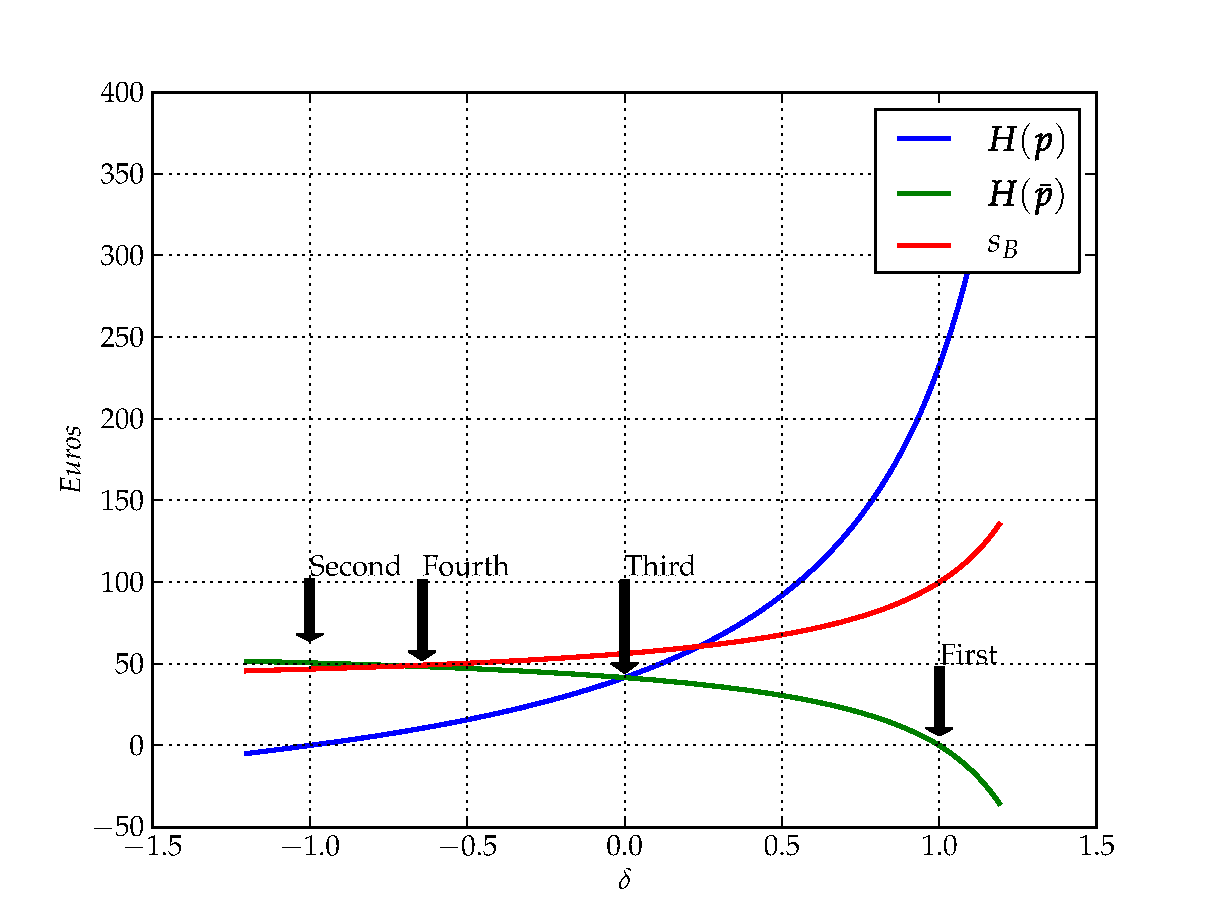
\includegraphics[width=0.8\linewidth]{imgs/biastrade.pdf}
\caption{Relation between the profits of problem
                                \ref{prb:backLayProblem} and $\delta$.}
\label{fig:biastrade}
\end{figure}

\bibliographystyle{plain}
\bibliography{bexchange}

\appendix
\section{Expected Value and Variance}
\label{apdx:expectedvariance}
First we need to suppose a value to the real probability that the event will happen, $P$. Normally a simple solution is to use the implicit probability that the market has established for the event at that moment. More complex approaches can be made with the retrieval of probabilistic information from external sources to the exchange or with the estimation of a trend of the market.

The expected value of a bet is colloquially called the value of the bet.

\subsection{Back}
The expected value of a back bet with real probability $P$ is:
\[
E \left[ Back(p_{B},s_{B}) \right] = \mu_{B} = P \times s_{B}
\frac{1-p_{B}}{p_{B}} - (1-P) \times (s_{B}) = s_{B}
                                       \left( \frac{P}{p_{B}}-1 \right)
\]
The variance is:
\[
Var \left[ Back(p_{B},s_{B}) \right] = P \left(
s_{B}\frac{1-p_{B}}{p_{B}} - \mu_{B} \right)^{2} + (1-P) \left( 
                                          - s_{B} - \mu_{B} \right)^{2}
\]

\subsection{Lay}
The expected value of a lay bet with probability $P$ is:
\[
E \left[ Lay(p_{L},s_{L}) \right] = \mu_{L} = P \times s_{L}
\frac{p_{L}-1}{p_{L}} + (1-P) \times (s_{L}) = s_{L} \left( 1 -
                                                \frac{P}{p_{L}} \right)
\]
The variance is:
\[
Var \left[ Lay(p_{L},s_{L}) \right] = P \left( s_{L}
\frac{p_{L}-1}{p_{L}} - \mu_{L} \right)^{2} + (1-P) \left( s_{L} -
                                                    \mu_{L} \right)^{2}
\]

\section{Back-Lay Commission Simplification}
\label{apdx:alphaone}
Observing the behaviour of $H$ in equation \ref{eq:tradingeq}, the 
following conditions are easily noted:

$$
    \left\{
    \begin{array}{l}
        C_{1}: s_{L} > s_{B}\\
        C_{2}: \frac{1-p_{B}}{p_{B}}s_{B} > \frac{1-p_{L}}{p_{L}}s_{L} \\
    \end{array} \right.
$$

Equation \ref{eq:tradingeq} can now be rewritten in the following way:

\begin{equation}
\label{eq:alphaBetaTrading}
    \alpha \times \beta \times\left( s_{L}-s_{B}\right) =
                \frac{1-p_{B}}{p_{B}}s_{B} + \frac{p_{L}-1}{p_{L}}s_{L}
\end{equation}
where $\alpha$ is
$$
    \left\{
    \begin{array}{c l}
        (1-h)         & \quad \text{if } C_{1} \wedge \bar{C_{2}}\\
        \frac{1}{1-h} & \quad \text{if }\bar{C_{1}} \wedge C_{2} \\
        1             & \quad \text{if }( C_{1} \wedge C_{2} ) \vee ( \bar{C_{1}} \wedge \bar{C_{2}} )\\
    \end{array} \right.
$$

The problem now is that $C_{1}$ and $C_{2}$ depend on the values of 
the stakes, which are the values we are trying to model. This said, 
both conditions will be solved in order to the implicit 
probabilities. Equation \ref{eq:alphaBetaTrading} can be simplified 
to the following form:
$$
s_{L} \times \left( \alpha \beta + \frac{1-p_{L}}{p_{L}} \right) =
s_{B} \times \left( \alpha \beta + \frac{1-p_{B}}{p_{B}} \right)
                                                        \Leftrightarrow
s_{L} = s_{B} \frac{ \alpha \beta + \frac{1-p_{B}}{p_{B}} }{ \alpha
                                        \beta + \frac{1-p_{L}}{p_{L}} }
$$

The first condition becomes:
$$
    s_{L} > s_{B} \Leftrightarrow
    s_{B} \frac{ \alpha \beta + \frac{1-p_{B}}{p_{B}} }{ \alpha \beta +
                        \frac{1-p_{L}}{p_{L}} } > s_{B} \Leftrightarrow
    \alpha \beta + \frac{1-p_{B}}{p_{B}}  > \alpha \beta +
                                  \frac{1-p_{L}}{p_{L}} \Leftrightarrow
    p_{L} > p_{B}
$$

And the second:
$$
    \frac{1-p_{B}}{p_{B}}s_{B} > \frac{1-p_{L}}{p_{L}}s_{L}
                                                        \Leftrightarrow
    \frac{1-p_{B}}{p_{B}} \left( \alpha \beta + \frac{1-p_{L}}{p_{L}}
    \right) > \frac{1-p_{L}}{p_{L}} \left( \alpha \beta +
                         \frac{1-p_{B}}{p_{B}} \right)  \Leftrightarrow
$$
$$
    \Leftrightarrow \alpha \beta \times \frac{1-p_{B}}{p_{B}} > \alpha
                     \beta \times \frac{1-p_{L}}{p_{L}} \Leftrightarrow
    p_{L} > p_{B}
$$

Concluding that $C_{1} \Leftrightarrow C_{2}$ which tells us that 
$\alpha=1$.
\end{document}
